\chapter{Theoretical Foundations}\label{ch:theoretical-foundations}

% ===============
% LEARNING FROM DATA
% ===============

\section{Learning from Data}

\subsection{Supervised vs Unsupervised Training}

TODO

\subsection{Backpropagation}

TODO

\subsection{Optimizer and Learning Rate}

TODO

\subsection{Automatic Evaluation}

Evaluating summaries is essential for multiple reasons, \eg to monitor progress during training or to compare own results to results from other researchers.
While human evaluation seems like an obvious approach, it is usually not feasible as it is slow, expensive and results from different people are not always comparable.
The more common approach is automatic evaluation.
To automatically evaluate summaries, ROUGE (Recall-Oriented Understudy for Gisting Evaluation) \cite{lin-2004-rouge} is widely adapted, as it tends to correlate well with human judgments.
ROUGE supports multiple evaluation metrics.
To report the results achieved in this thesis, the following three metrics are used:
\begin{itemize}
\item \textbf{ROUGE-1} which calculates the overlap of single words (unigrams) between the candidate summary and the reference summary. 
\item \textbf{ROUGE-2} which is similar to ROUGE-1, but instead of using the overlap of single words, it uses word pairs of 2 (bigram).
\item \textbf{ROUGE-SU4} which uses a combination of unigram overlap and skip-4gram overlap.
A skip-4gram is an ordered pair of 4 words, ignoring any gaps between the words.
\end{itemize}

When comparing word overlap, one has to differentiate between recall and precision \cite{Ting2010}.
While recall indicates, how much information of the reference summary is present in the candidate summary, precision indicates how much of the information in the candidate summary is actually present in the reference summary.
It is common to combine these two measures to a single one, that is called F1-measure.
It is calculated by the following formular:
\[
	F_1 = 2 \cdot \frac{Recall \cdot Precision}{Recall + Precision}
\]

% ==========
% TRANSFORMER
% ==========

\section{Transformer}\label{sec:transformer}

The Transformer is a neural network architecture for sequence learning that was published in 2017 \cite{1706.03762}.
It achieved new state-of-the-art results for many machine translation tasks while at the same time requiring significant less training time compared to previous well performing models.

\subsection{Motivation}\label{ssec:transformer-motivation}

In the recent years, recurrent neural networks (RNNs) have been the most common way to solve sequence learning tasks.
One of the big downsides of RNNs is its sequential behaviour.
To train a RNN, the elements of the input sequence are fed into the neural network one after another.
While the sequence elements are passed through the RNN, a hidden state gets computed at every step, that is part of the input for the next step.
This process is called encoding.
Afterwards, the last hidden state of the econding process is used as an input for the first step of the decoding process.
Because of this, it is not possible to parallelize the training within a training example, as the hidden state of the previous step is needed to calculate the output of the current step. \cite[p.~2]{1706.03762}
A simplified RNN for sequence-to-sequence tasks like machine translation is shown in \cref{fig:rnn-visualization}.

\begin{figure}[h]
\centering
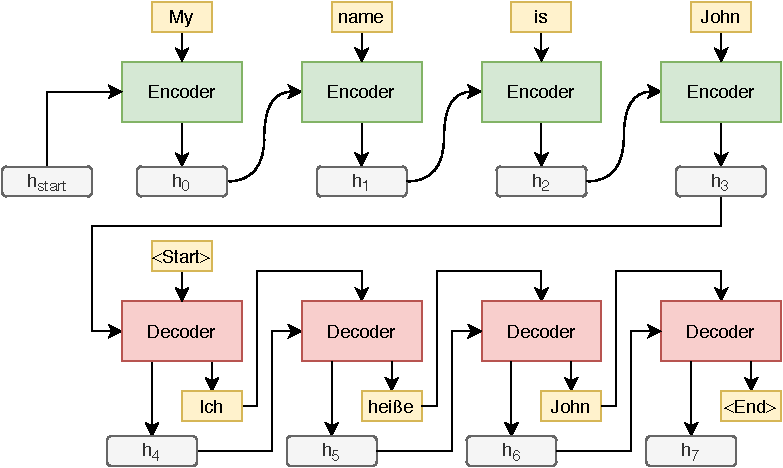
\includegraphics{figures/rnn-visualization}
\caption[Simplified visualization of a sequence-to-sequence RNN network for machine translation]{Simplified visualization of a sequence-to-sequence RNN network for machine translation. The input sequence is fed into the Encoder with one word each step. The final hidden state, that is computed in the last encoding step, is used as input for the first decoding step. The initial hidden state $h_{start}$ can be initialized as a vector of zeros or learned during training.}
\label{fig:rnn-visualization}
\end{figure}

Another problem of RNNs is the long distance, information has to "travel" before it is used.
Information that was encoded into the hidden state has to pass through multiple encoding and decoding steps, before it is finally used in one of the decoding steps.
Besides having the hidden state as an information bottleneck, this also makes it very hard for the network to learn long range dependencies because of the problem of vanishing or exploding gradients \cite{Hochreiter01gradientflow}.
Modern variants of RNNs like the long short-term memory (LSTM) architecture \cite{Hochreiter1997} try to mitigate these effects, but aren't able to fully eliminate them.
A fairly recent solution to this problem is the attention mechanism, that was first proposed in 2014 \cite{1409.0473}.
It allows the network in the decoding stage to retrieve information from any hidden state that was computed during the encoding stage.
This eliminates the problem of learning long range dependencies.

The Transformer network tries to take advantage of the attention mechanism while ditching the recurrence of RNNs to achieve faster training and allow for more parallelization.

\subsection{Model Architecture}\label{ssec:transformer-model-architecture}

Just like sequence-to-sequence RNNs, the Transformer consists of an encoder and a decoder that both consist of a stack of layers.

\begin{figure}[h]
\centering
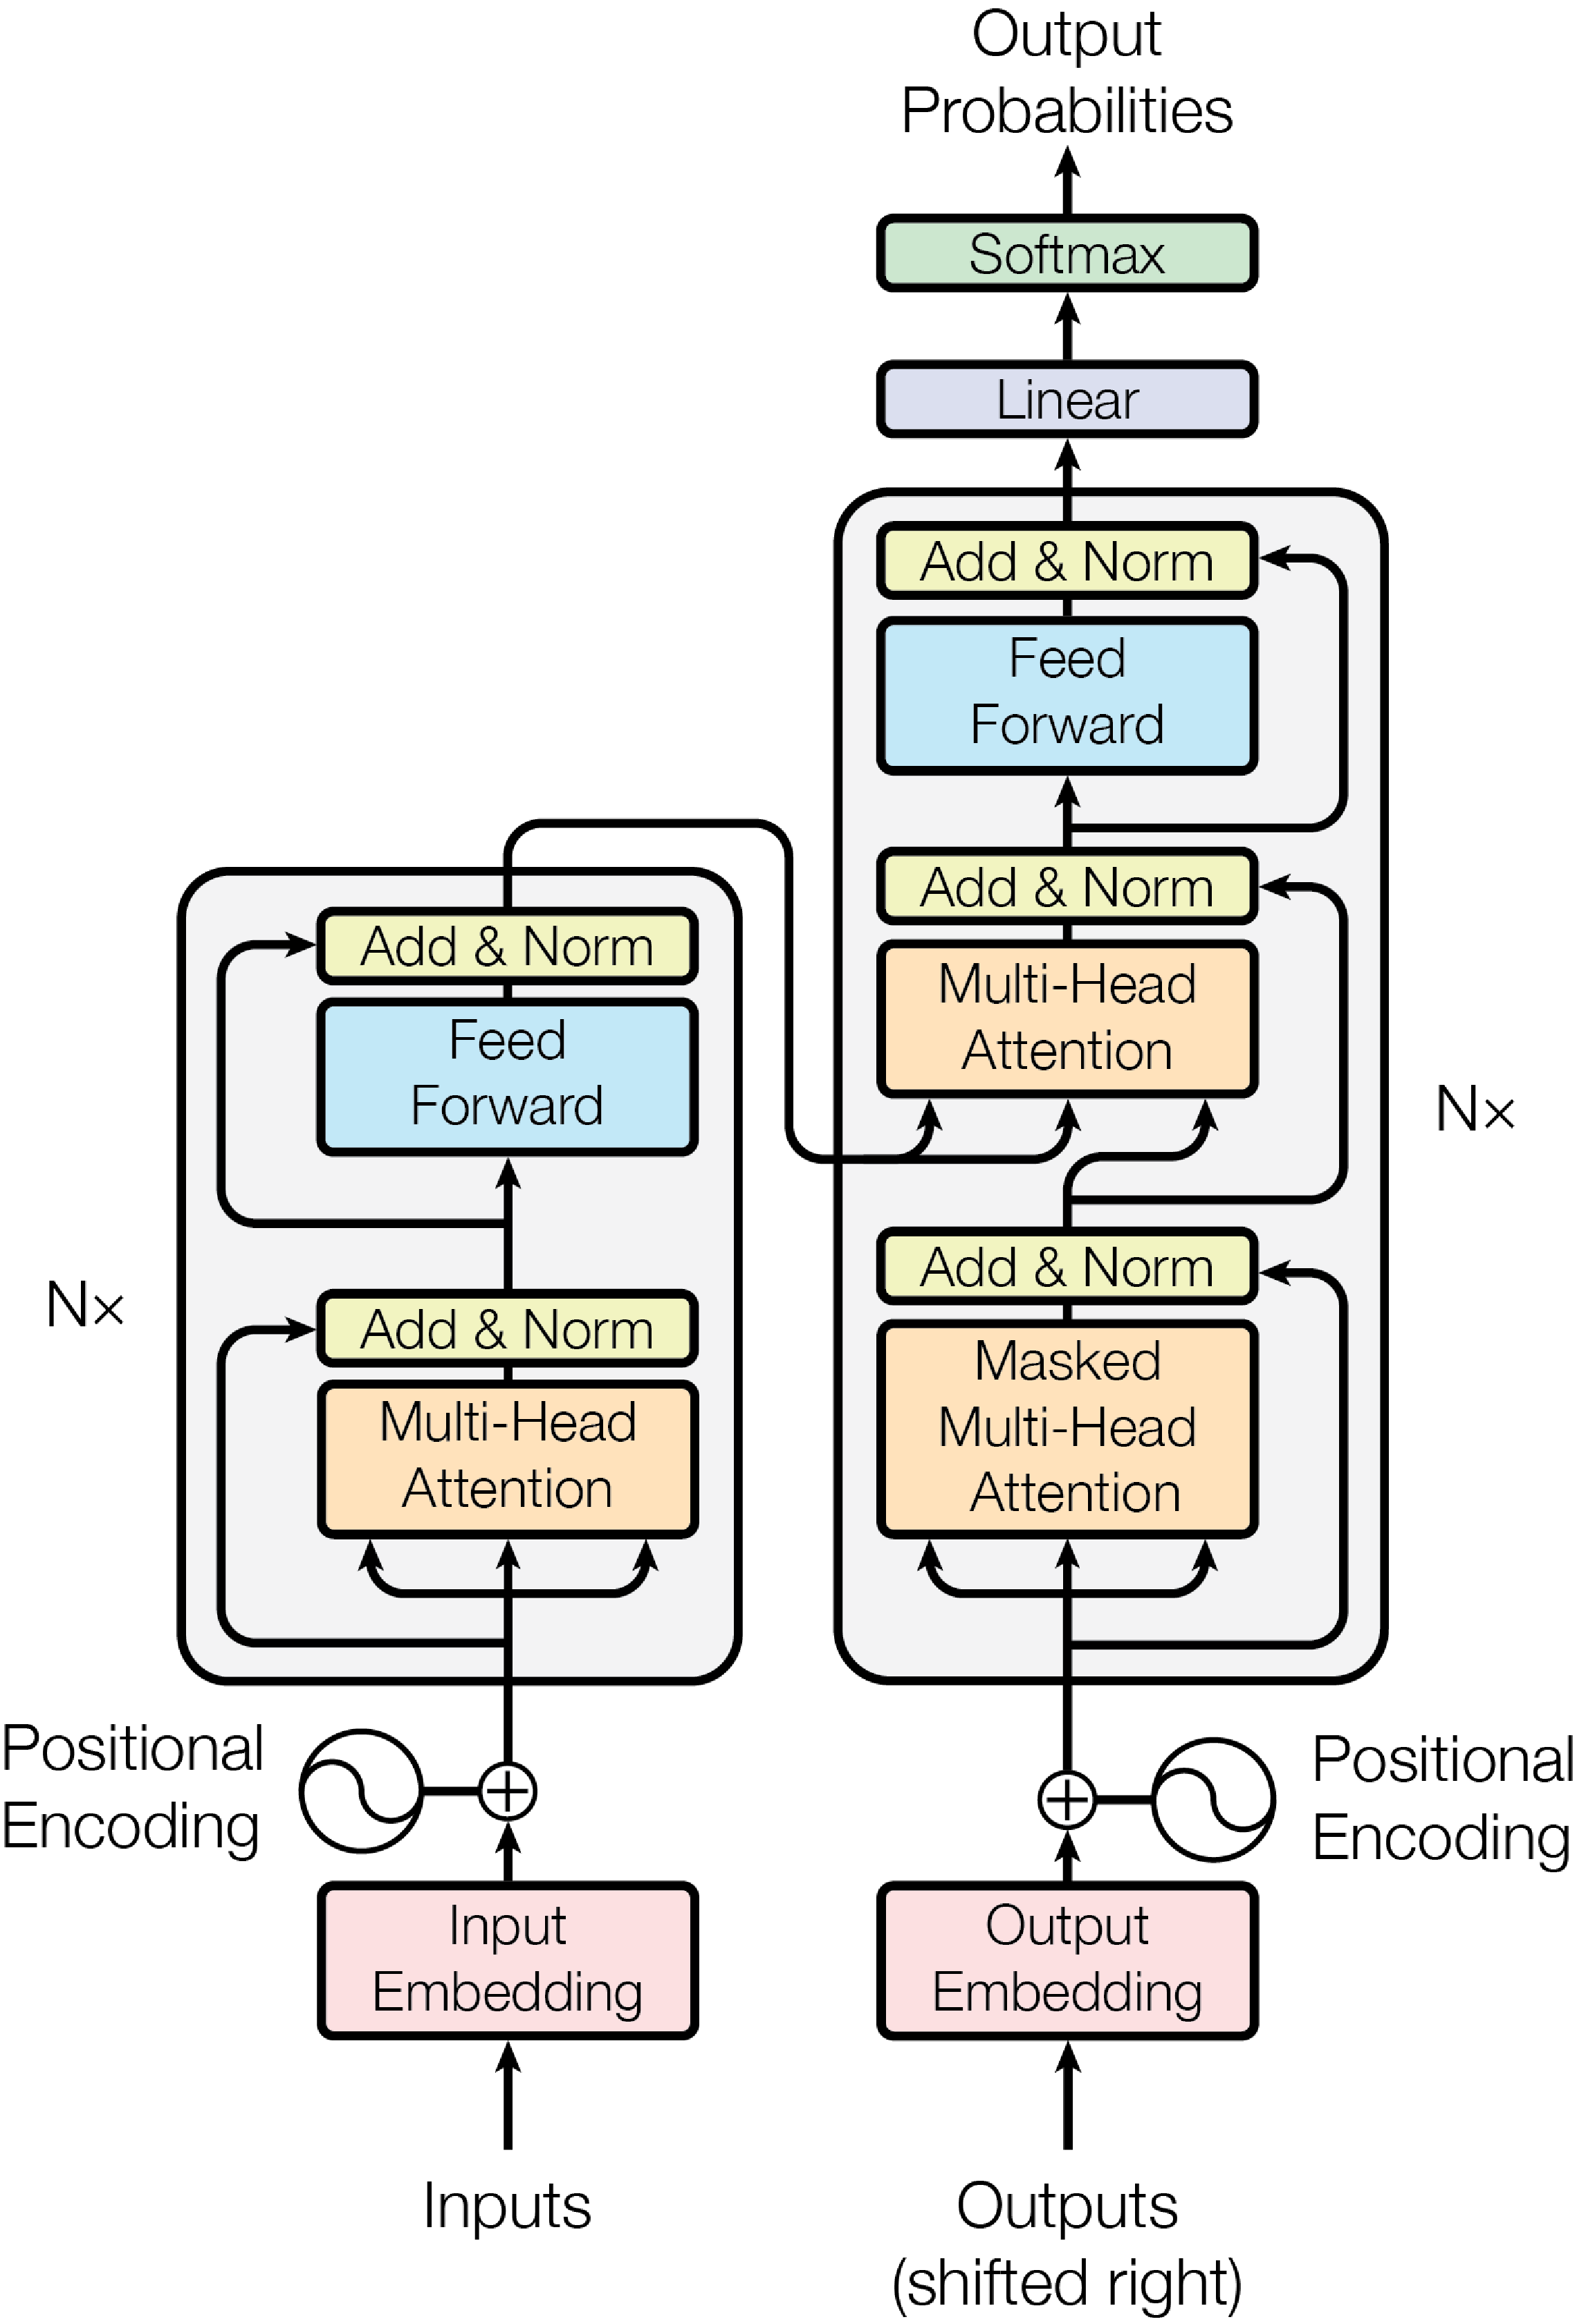
\includegraphics{figures/transformer-model}
\caption[Model architecture of a Transformer]{Model architecture of a Transformer \cite[p.~3]{1706.03762}.}
\label{fig:transformer-model}
\end{figure}

An encoder layer consists of two sub-layers.
The first sub-layer is a multi-head self-attention mechanism which is described later in this section.
The second sub-layer is a position-wise \footnote{The identically network is applied to each position separately \cite[p.~5]{1706.03762}} fully connected feed-forward network.
Both sub-layers have residual connections \cite{1512.03385} around them, that are followed by layer normalization \cite{1607.06450}.
The outputs of the layers of the Transformer base model have $d_{model}=512$ dimensions and $d_{model}=1024$ for the big model \cite[p.~9]{1706.03762}.

The encoder layer has a similar structure, but with one additional sub-layer and a slight modification of the multi-head self-attention sub-layer.
The new sub-layer is able to attend to the output of the encoder.
The multi-head self-attention sub-layer is masked, to prevent it from attending to future words. \cite[p.~3]{1706.03762}.

In the original Transformer, $N = 6$ stacked encoder and decoder layers are used.
The complete architecture of the Transformer is visualized in \cref{fig:transformer-model}.

The inputs are simple learned embedding vectors of dimension $d_{model}$ that are concatenated with a fixed positional embedding \cite[p.~5--6]{1706.03762}.
This fixed input embeddings encode the position of the sequence elements, as this information is otherwise no longer accessible to the network because of the missing recurrence.
The positional encoding is calculated with sine and cosine functions of different frequencies:
\begin{align*} 
	PE_{(pos,2i)} & = sin(pos/10000^{2i/d_{model}}) \\
	PE_{(pos,2i+1)} & = cos(pos/10000^{2i/d_{model}})
\end{align*}

This encoding allows the network to obtain information about the absolute and relative position of each element.
\Cref{fig:positional-encoding-sine-cosine} visualizes the embedding for some dimensions.
It is clearly visible how each position has a different embedding.

For the outputs, a learned linear transformation and a softmax function are used to generate next-token probabilities \cite[p.~5]{1706.03762}.

\begin{figure}[h]
\centering
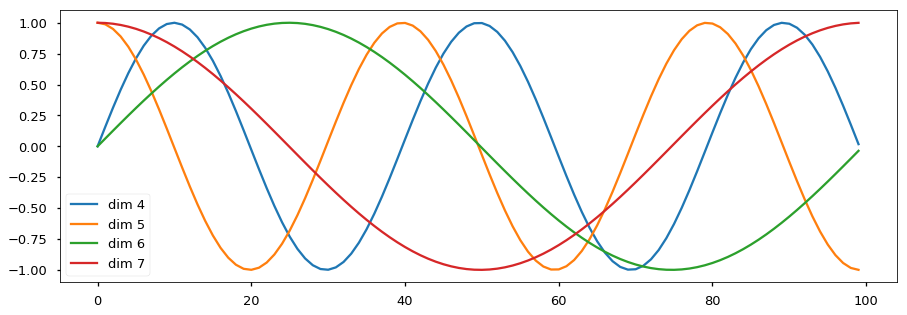
\includegraphics[width=0.7\paperwidth]{figures/positional-encoding-sine-cosine}
\caption[Visualization of positional encoding with sine and cosine]{Visualization of positional encoding with sine and cosine \cite{annotated.transformer}.}
\label{fig:positional-encoding-sine-cosine}
\end{figure}

\subsubsection{Attention}

\begin{figure}[h]
\centering
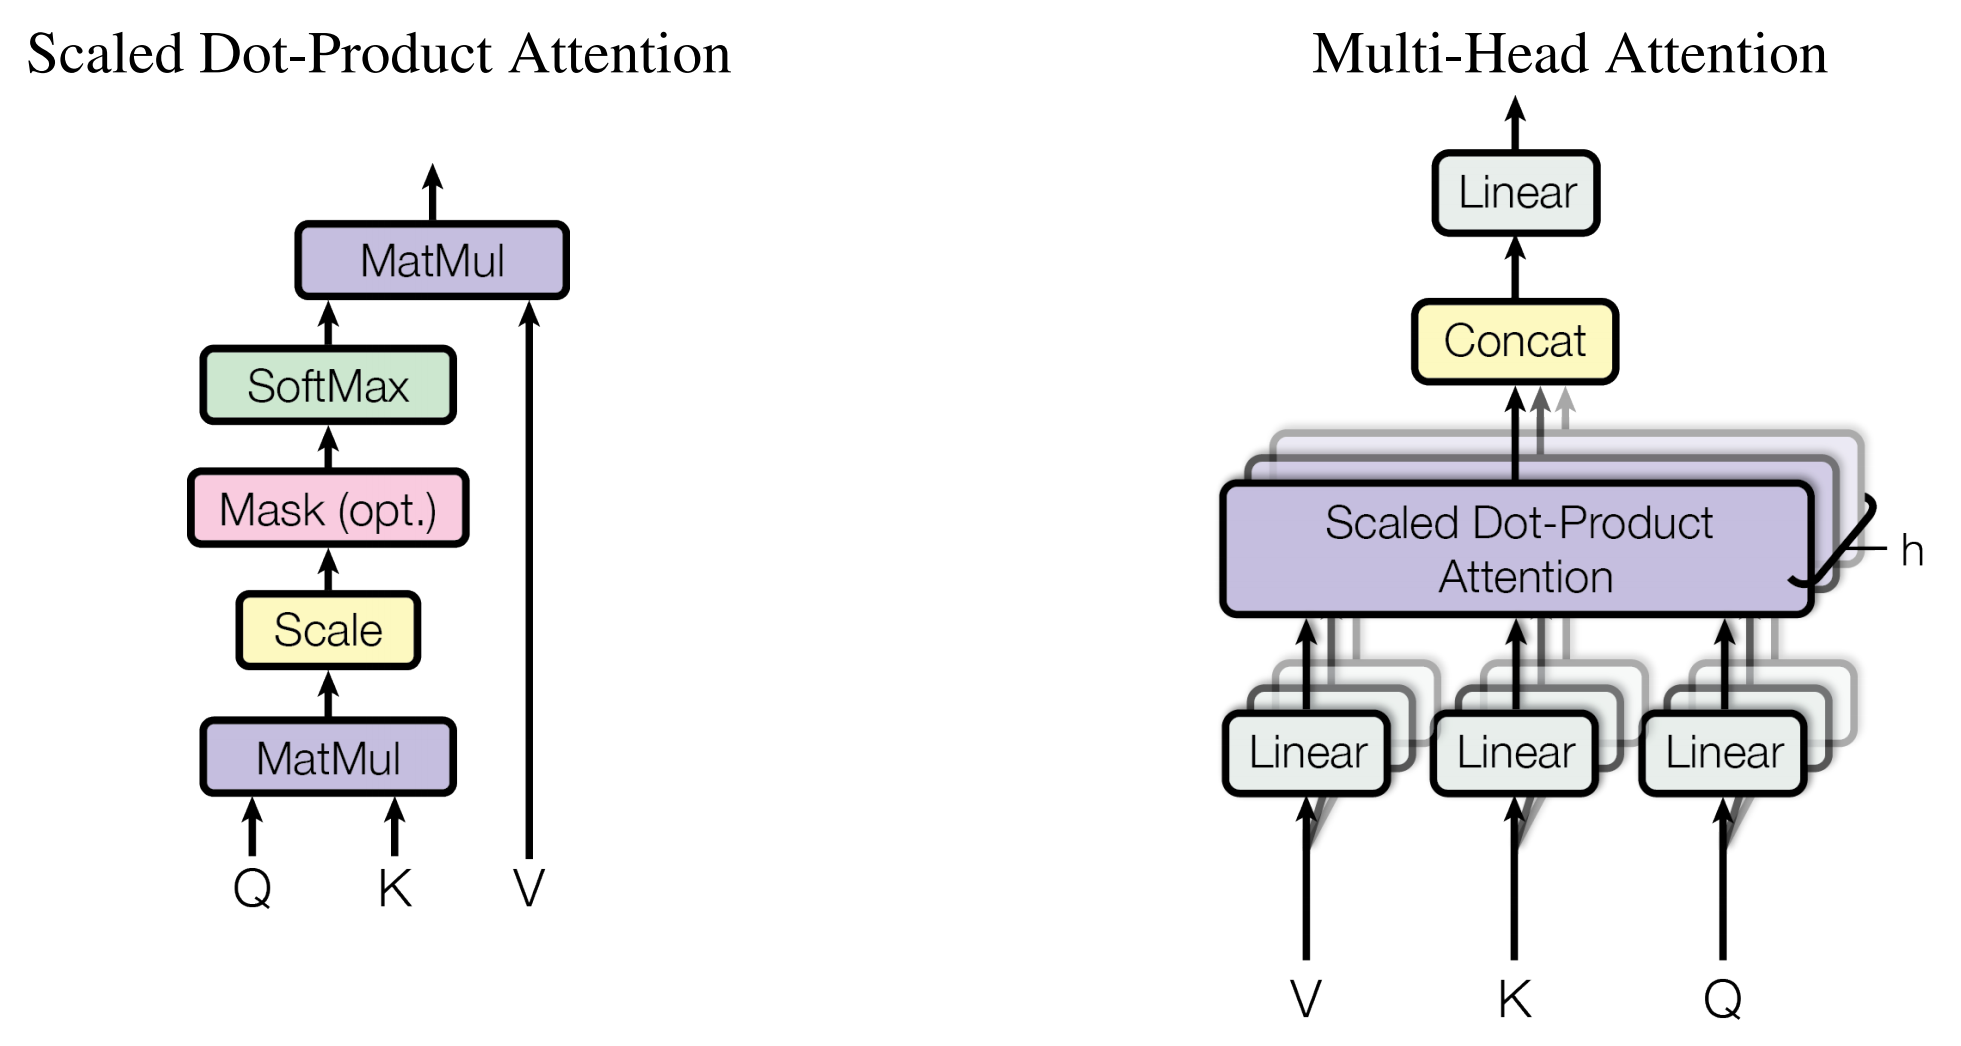
\includegraphics[width=0.7\paperwidth]{figures/scaled-dot-product-multihead-attention}
\caption[Visualization of Scaled Dot-Product Attention and Multi-Head Attention]{Visualization of Scaled Dot-Product Attention and Multi-Head Attention \cite[p.~4]{1706.03762}.}
\label{fig:scaled-dot-product-multihead-attention}
\end{figure}

The Transformer attention consists of query, key and value vectors.
The query vectors are used to select values by their corresponding keys.
The Transformer implements this as a "Scaled Dot-Product Attention" where queries and key have the dimension $d_k$ and the values the dimension $d_v$.
To calculate the attention, the following formula is used:
\[
	\textrm{Attention}(Q,K,V) = \textrm{softmax}(\dfrac{QK^T}{\sqrt{d_k}})V
\]
where the matrices $Q$, $K$ and $V$ contain multiple sets of queries, keys and values \cite[p.~3--4]{1706.03762}.

Unlike normal attention, the Transformer uses "Multi-Head Attention".
Instead of having a single attention function, the queries, keys and values are linearly projected with learned linear projections \cite[p.~4--5]{1706.03762}.
After performing the attention function on the projected matrices, they are concatenated and projected again.
The dimension of each learned linear projection is the model's dimension $d_{model}$ divided by the amount of attention layers $h$.
\Cref{fig:scaled-dot-product-multihead-attention} visualizes both the "Scaled Dot-Product Attention" (left) as well as the "Multi-Head Attention" (right).

\subsection{Advantages}

As described in \cref{ssec:transformer-motivation}, the Transformer allows for significant more parallelization than RNNs, because of the absence of sequential behavior within one training example.
This yields in much faster and less expensive training, compared to previous state-of-the-art models for machine translation.
The big Transformer model is trained for 3.5 days on 8 P100 GPUs and the base Transformer model for just 12 hours \cite[p.~7]{1706.03762}. 
For comparison, the first RNN network to utilize attention took between 109 and 252 hours for training \cite[p.~14]{1409.0473}.

\subsection{Disadvantages}

Transformer networks tend to get very large and require a lot of memory especially for longer sequence length, as the self-attention connects every position with every other position in the sequence.
This results in quadratic complexity for the sequence length.
As a solution, the authors of the Transformer suggest to limit the self-attention to the neighbors of each position \cite[p.~6--7]{1706.03762}.  
The more recent Reformer \cite{kitaev2020reformer} tries to solve the issues by using locality-sensitive hashing to reduce the complexity from $O(L^2)$ to $O(L)$.

% ====
% BERT
% ====

\section{BERT}\label{sec:bert}

BERT (\textbf{B}idirectional \textbf{E}ncoder \textbf{R}epresentations from \textbf{T}ransformers) is a general-purpose language model, that was released by Google AI researchers in mid 2018.
It broke several records for Natural Language Processing Benchmarks \cite[p.~5--7]{devlin2018bert}, such as  SQuAD v1.1 \cite{rajpurkar-etal-2016-squad} or GLUE \cite{1804.07461}.

\subsection{Motivation}

It has been shown, that results for many natural language processing tasks can be improved with the help of language models.
The most famous amoung them are OpenAI's GPT-2 \cite{radford2019language} and ELMo \cite{1802.05365}.
The benefit of language models is, that most of them can be trained on unlabeled data, like Wikipedia articles or large book corpora.
This allows them to learn from a huge amount of data, as there is no need for time-consuming labeling of the training data and any texts can be used.
By pre-training them on normal texts, the networks can get a general sense of natural language.
This general sense for language can then be used for more specific tasks.

% TODO Not sure if I keep using this or create an own one / just remove it
\begin{figure}[h]
\centering
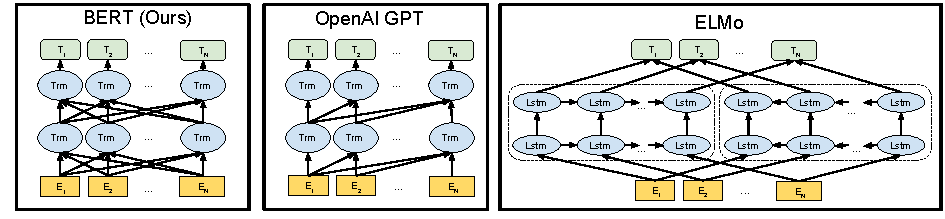
\includegraphics[width=0.7\paperwidth]{figures/bert-gpt2-elmo-model-comparison}
\caption[Visualisation of the different model architectures]{Visualisation of the different model architectures \cite[p.~13]{devlin2018bert}.}
\label{fig:bert-gpt2-elmo-model-comparison}
\end{figure}

What's new about BERT, compared to other models like GPT-2, is, that it is the first deeply bidirectional language model, that takes advantage of the whole context around of a word.
OpenAI's GPT-2 uses a left-to-right Transformer \cite[p.~4]{radford2019language}, which only allows it to "look" at the words to the left, when generating a representation for an input token.
For example, when having a sentence that starts with "The lighter", the network can only look at these two words to generate a representation for the word "lighter".
However, the word can have completely different meanings, depending on the whole sentence, e.g. "The lighter is an easy tool to make fire" compared to "The lighter shade of red looks better than the darker one". 
ELMo tries to compensate this issue by training two LSTMs with one being a normal forward LSTM (left-to-right) and the other one being a backward LSTM (right-to-left) which is given the input sequence in reverse \cite[p.~2--3]{1802.05365}.
Afterwards, it concatenates the representations of these two LSTMs to get a semi-bidirectional representation.
\Cref{fig:bert-gpt2-elmo-model-comparison} visualizes the different architectures.

\subsection{Model Architecture}

At its core, BERT is just a Transformer decoder, as described in \cref{ssec:transformer-model-architecture}.

\subsubsection{Input and Output Representations}

BERT's input tries to be applicable for many different natural language processing tasks.
It allows the inputs of either one sentence or a pair of two sentences, with sentences refering to ``an arbitrary span of contiguous text, rather than an actual linguistic sentence'' \cite[p.~4]{devlin2018bert}.
Texts are tokenized by using WorkPiece embeddings with a vocabulary of 30'000 tokens. % TODO Maybe explain the tokenization in more detail
Every input sequence starts with a special \texttt{[CLS]} token and every sentence ends with a special \texttt{[SEP]} token.
Additionally to the token embeddings, the input consists of two more types of embeddings.
The first one are a learned segment embeddings, that indicates if a token belongs to the first or the second token.
The second one are position embeddings, that help the network to understand the positions of each token in the sequence.
Unlike the original Transformer, BERT does not use fixed posisional embeddings, but learned ones.
Finally, these three embeddings are concatendated to form the actual input for the network as shown in \cref{fig:bert-input-representation}.

\begin{figure}[h]
\centering
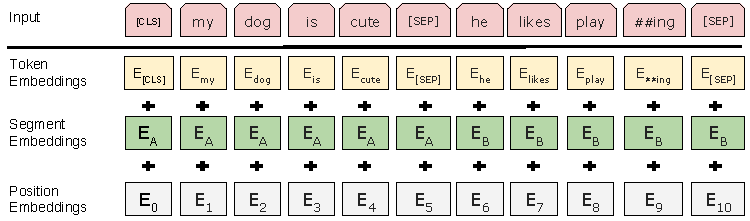
\includegraphics{figures/bert-input-representation}
\caption[BERT input representation]{BERT input representation \cite[p.~5]{devlin2018bert}.}
\label{fig:bert-input-representation}
\end{figure}

Depending on the task to perform, there are different ways to use the final hidden states of the BERT Transformer network.
For sentence classification tasks, the \texttt{[CLS]} token representation can be used.
This work uses the final hidden states for every single input token, as the Decoder should have access to the presentation of every input token.
For the simpler extractive summarization task, which is basically some kind of sentence classification in which each sentence is either classified as \texttt{"include in summary"} or \texttt{"do not include in summary"}, it can be sufficient to only use the final hidden state of the \texttt{[CLS]} token. 
\cite{1903.10318} proposes a small input variation for BERT, that inserts multiple \texttt{[CLS]} tokens into the input sequence to later use them for extractive summarization.

\subsubsection{Pre-Training Objectives}

BERT is pre-trained with two different tasks \cite[p.~4--5]{devlin2018bert}.
For the first task, the network is given a sentence with 15\% of its word piece tokens b randomly masked.
An example for masking is shown in \cref{fig:bert_masking_example}.

% TODO Exact source is https://github.com/google-research/bert#what-is-bert
% TODO I need to ask my prof if the current mentioning of the GitHub page is enough
\begin{figure}[h]
\begin{lstlisting}[numbers=none]
Input: the man went to the [MASK1] . he bought a [MASK2] of milk.
Labels: [MASK1] = store; [MASK2] = gallon
\end{lstlisting}
\caption[Masked input example]{Masked input example. Taken from the BERT GitHub page.}
\label{fig:bert_masking_example}
\end{figure}


The task of the network is, to predict the masked tokens.
This task allows the network to take the context of a word into consideration.

For the second task, the network is given two sentences.
The network then has to predict, if the second of these two sentences comes after the first one in the original text or if it is just a randomly selected sentence from any other text.
An example for next sentence prediction is shown in \cref{fig:bert_next_sentence_example}.

% TODO Exact source is https://github.com/google-research/bert#what-is-bert
% TODO I need to ask my prof if the current mentioning of the GitHub page is enough
\begin{figure}[h]
\begin{lstlisting}[numbers=none]
Sentence A: the man went to the store .
Sentence B: he bought a gallon of milk .
Label: IsNextSentence

Sentence A: the man went to the store .
Sentence B: penguins are flightless .
Label: NotNextSentence
\end{lstlisting}
\caption[Next sentence prediction example]{Next sentence prediction example. Taken from the BERT GitHub page.}
\label{fig:bert_next_sentence_example}
\end{figure}

Ideally, this helps the network to understand the relationship between two sentences.
However, this task has been shown to be too simple for the network, as it is easier for it to just learn if the topics of two sentences match instead of understanding the real relationship of the sentences.
Newer successors of BERT such as ALBERT use slightly changed training objectives, like sentence order prediction \cite[p.~3]{1909.11942} in which the goal is to predict, which of two given sentences comes first.

Pre-training is usually very expensive.
The training was performed for 4 days on 4 Cloud TPUs for BERT\textsubscript{BASE} and 16 Cloud TPUs for the larger model BERT\textsubscript{LARGE} with each Cloud TPU having 4 TPU chips \cite[p.~13]{devlin2018bert}.
However, it is only necessary to do pre-training once.

\subsubsection{Fine-Tuning}

After the unsupervised pre-training, the network can be fine-tuned for a specific task.
Fine-Tuning is far less expensive than pre-training and can usually be done in less than 1 hour on a single Cloud TPU, or a few hours on a normal GPU \cite[p.~5]{devlin2018bert}.
% TODO This chapter can be a bit longer...